\begin{figure}[ht]\centering
% KB's picture, redone in tikz below to change text
%  \includegraphics[width=0.5\textwidth]{images/mathematical-data.pdf}
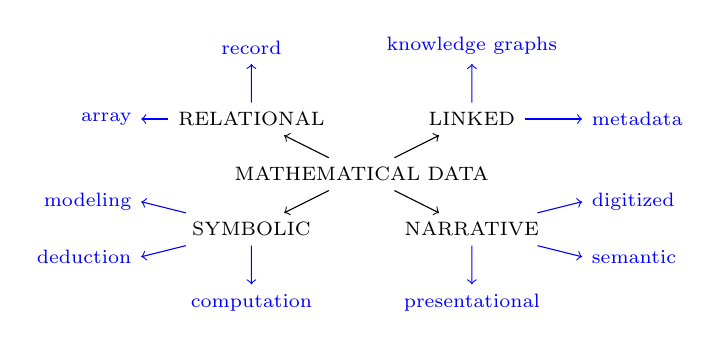
\begin{tikzpicture}
\begin{scope}[font=\scriptsize,scale=.7]
\begin{scope}[]
\node (m) at (0,0) {MATHEMATICAL DATA};
\end{scope}
\begin{scope}[]
\node (s) at (-2,-1) {SYMBOLIC};
\node (r) at (-2,1) {RELATIONAL};
\node (l) at (2,1) {LINKED};
\node (n) at (2,-1) {NARRATIVE};
\draw[->] (m) -- (s);
\draw[->] (m) -- (l);
\draw[->] (m) -- (r);
\draw[->] (m) -- (n);
\end{scope}

\begin{scope}[blue]
\draw[->] (r) -- ++(0,1) node[above] {record};
\draw[->] (r) -- ++(-2,0) node[left] {array};
\draw[->] (l) -- ++(0,1) node[above] {knowledge graphs};
\draw[->] (l) -- ++(2,0) node[right] {metadata};
\draw[->] (s) -- ++(-2,.5) node[left] {modeling};
\draw[->] (s) -- ++(-2,-.5) node[left] {deduction};
\draw[->] (s) -- ++(0,-1) node[below] {computation};
\draw[->] (n) -- ++(2,0.5) node[right] {digitized};
\draw[->] (n) -- ++(2,-.5) node[right] {semantic};
\draw[->] (n) -- ++(0,-1) node[below] {presentational};
\end{scope}
\end{scope}
\end{tikzpicture}
\caption{Kinds of mathematical data}\label{fig:mathematical-data}
\end{figure}

In order to better analyze the current state of the art of FAIRness in mathematical data, we introduce a novel categorization of mathematical data.
An overview is given in Figure~\ref{fig:mathematical-data}.
Each kind of data makes different abstractions or focuses on different aspects of mathematical reality, resulting in characteristic strengths and weaknesses.
We summarize these in Figure~\ref{fig:datakinds}.

\begin{figure}[hbt]\centering\footnotesize
\begin{tabular}{|p{3.5cm}|cccc|}\hline
Kind of data & Sym. & Rel. & Lin. & Nar.\\\hline
Machine-understandable  & \textbf{+} & \textbf{+} & \textbf{+}& \textbf{--}\\
Complete description & \textbf{+} & \textbf{+} & \textbf{--}& \textbf{+}\\
Applicable to all objects & \textbf{+} & \textbf{--} & \textbf{+}& \textbf{+}\\
Easy to produce  & \textbf{--} & \textbf{+} & \textbf{+}& \textbf{+}\\
\hline
\end{tabular}
\caption{Advantages of different kinds of data}\label{fig:datakinds}
\end{figure}

\paragraph{Symbolic data} consists of formal expressions such as formulas, formal proofs, programs, etc.
These are written in a variety of highly-structured formal languages specifically designed for individual domains and with associated tools.
The most important such domains are \textbf{modeling}, \textbf{deduction}, and \textbf{computation} employing modeling languages, logics, resp. programming languages.
The associated tools like simulation tools, proof assistants, resp. computer algebra systems can understand the entire semantics of the data.

Because symbolic data allows for abstraction principles such as underspecification, quantification, and variable binding, it can capture the complete semantics of any mathematical object.
However, the formalization of a typical narrative theorem as a statement in a proof assistant or a function in a computer algebra system can be very expensive.
This comes at the price of being context-sensitive: expressions cannot be easily moved across environments, which makes \emph{Finding}, \emph{Reusing}, and \emph{Interoperability} difficult.

Moreover, because each tool usually defines its own formal language and because these are usually mutually incompatible, interoperability and reuse across these individual tools are practically non-existent.
To overcome this problem, multiple representation formats have been developed for symbolic data, usually growing out of small research projects and reaching different degrees of standardization, tool support, and user following.
These are usually optimized for specific applications, and little cross-format sharing is possible.
In response to this problematic situation, standard formats have been designed such as MathML~\cite{CarlisleEd:MathML3:on} and OMDoc/MMT~\cite{uniformal:on}.
%The latter has been used as an interoperability format for computer algebra systems in the OpenDreamKit project and already offers comprehensive services for symbolic data such as querying. 

\paragraph{Relational data} employs representation theorems that allow encoding mathematical objects as ground data built from numbers, strings, tuples, lists, etc.
Thus, relational data combines optimized storage and processing with capturing the whole semantics of the objects.
It is also easy to produce and curate as general purpose database technologies and interchange formats such as CSV or JSON are readily available.

Relational datasets can be subdivided based on the structure of the entries, which often enable different optimized database solutions.
The most important ones are record data, where datasets are sets of records conforming to the same schema and which are stored in relational databases, and \textbf{array} data, which consists of very large, multidimensional arrays stored in optimized array databases. %% tree and graph data?
%Array data tends to come up in settings with large but simply-structured datasets such as simulation time series, while record data is often needed to represent complex objects, especially those from pure mathematics.

However, these representation theorems do not always exist because sets and functions, which are the foundation of most mathematics, are inherently hard to represent concretely.
Moreover, the representation theorems may be very difficult to establish and understand, and there may be multiple different representations for the same object.
Therefore, applicability is limited and must be established on a case by case basis.

Therefore, \emph{Interoperability} is difficult because users need to know the exact representation theorem and the exact way how it is applied to understand the encoding.
Therefore, even if the representation function is documented, \emph{Finding}, \emph{Reuse}, and \emph{Interoperability} are theoretically difficult, practically expensive, and error-prone.
For example, consider the following very recent incident from (Jan. 2019): 
There are two encoding formats for directed graphs, both called \texttt{digraph6}: Brendan McKay's \cite{McKayFormats:on} and the one used by the GAP package Digraphs \cite{GAPDigraphFormat:on}, whose authors were unaware of McKay's format and essentially reinvented a similar one \cite{digraph6issue:on}.
The resulting problem has since been resolved but not without causing some misunderstandings first.

\paragraph{Linked data} introduces identifiers for objects and then treats them as blackboxes, only representing the identifier and not the original object.
The internal structure and the semantics of the object remain unspecified except for maintaining a set of named relations and attributions for these identifiers.
This abstraction allows for universal applicability at the price of not representing the complete mathematical object.

The named relations allow forming large networks of objects, and the attributions of concrete values provide limited information about each one.
Linked data can be subdivided into \textbf{knowledge graphs} based on mathematical ontologies and \textbf{metadata}, e.g., as used in publication indexing services.

As linked data forms the backbone of the Semantic Web, linked data formats are very well-standardized: data formats come as RDF, the relations and attributes are expressed as ontologies in OWL2, and RDF-based databases (also called triplestores) can be queried via SPARQL.
For example, services like DBPedia and Yago crawl various aspects of Wikipedia to extract linked data collections and provide SPARQL endpoints.
%They supply a valuable fallback for the linked data ontologies to be developed in the \pn project.
The WikiData database~\cite{wikidata:on} collects such linked data and uses them to answer queries about the objects.
%This makes WikiData a primary target for the purposes of linked data management in \pn. 

Thus, contrary to, linked data has very good FAIR-readiness, in particular allowing for URI-based \emph{Access}, efficient \emph{Finding} via query languages, and URI-mediated \emph{Reuse} and \emph{Interoperability}.
%For example, it is general practice to use the URIs of the respective Wikipedia articles unless more specific ontologies are available.
However, this FAIR-readiness comes at the price of not capturing the complete semantics of the objects so that \emph{Access} and \emph{Finding} are limited and \emph{Interoperability} and \emph{Reuse} are subject to misinterpretation.


\paragraph{Narrative data} consists of mathematical documents and text fragments. We speak of \textbf{mathematical vernacular} for the peculiar mixture of mathematical formulae, natural language with special idioms, and diagrams. There are four levels of formality of narrative data:
\begin{compactenum}
\item \textbf{digitized:} scanned into images from documents,
\item \textbf{presentational:} represented in a form that allows flexible
  presentation on electronic media, such as web browsers;
  born digital or OCRed from digitized ones,
\item \textbf{semantic}: in a form that makes explicit the functional structure and the
  relations between formulae, the objects they denote and the mathematical context.
\end{compactenum}
All levels of formality are relevant for mathematical communication, but machine support for reasoning and knowledge management can only be given at the semantic level.
We could extend this classification by a fourth level of narrative data for formalized documents; but these abstract from the narrative form and are therefore counted as symbolic data.

Note that we can always go from higher levels to lower ones, by styling: presenting semantic features by narrative patterns. Therefore we also count such patterns as narrative data -- e.g. \textbf{notation definitions} such as $\left(n\atop k\right)$ or $\mathcal{C}^n_k$ for the binomial coefficients or verbalizations in different languages.

%%% Local Variables:
%%% mode: latex
%%% mode: visual-line
%%% fill-column: 5000
%%% TeX-master: "report"
%%% End:

%  LocalWords:  centering includegraphics textwidth inparahighlight categorization analyzing summarized ednote hline textbf textbf textbf textbf emph emph emph standardization optimized texttt triplestores LehIseJak:dlsmkbew13 HofSucBer:yago2a analyze formalization digitized calbf verbalizations
